\newpage		
	\section*{Лист 4}
		\subsection*{1-2}
		\noindent
		Заметим что замощение плоскости можно определить через пару $(p,q)$, где $p$ -- количество вершин многоугольника которым замощается плоскость, а $q$ -- количество многоугольников касающихся друг друга в каждой из вершин.
		\vskip 0.1in
		\noindent
		Тогда можно вывести сумму углов каждого многоугольника, зная $(p,q)$: $p \cdot \frac{2 \pi}{q}$. Тогда можно заметить, что сумма углов будет являться произведением $2\pi$ и некой дроби $\frac{p}{q},\ p,q \in \mathbb{N}$.
		\vskip 0.1in
		\noindent
		Вернемся к задаче, так как мы рассматриваем замощение четырехугольниками, то $p = 4$, следовательно все возможные углы можно представить как $\frac{8\pi}{q}$, откуда следует что при $q = 8$ можно получить сумму углов $\pi$, а при $q=32$ можно получить $\frac{\pi}{4}$, также становится очевидным то, что сумму углов $\frac{\pi}{\sqrt{2}}$ получить невозможно, так как $\frac{1}{\sqrt{2}}$ нельзя представить как $\frac{a}{b},\ a,b \in \mathbb{N}$\\
		Ответ: a) да, б) да, в) нет
		\begin{figure}[h!]
			\begin{minipage}[h]{0.5\linewidth}
				\center{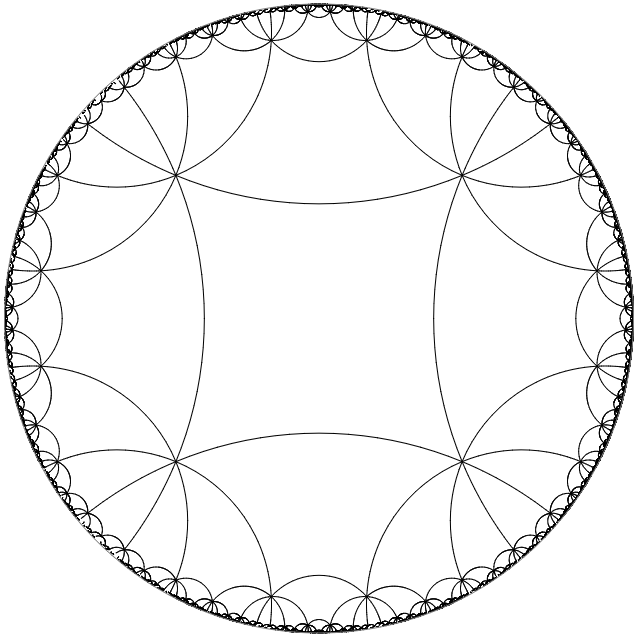
\includegraphics[width=0.8\linewidth]{pic12}}
			\end{minipage}
			\hfill
			\begin{minipage}[h]{0.5\linewidth}
				\center{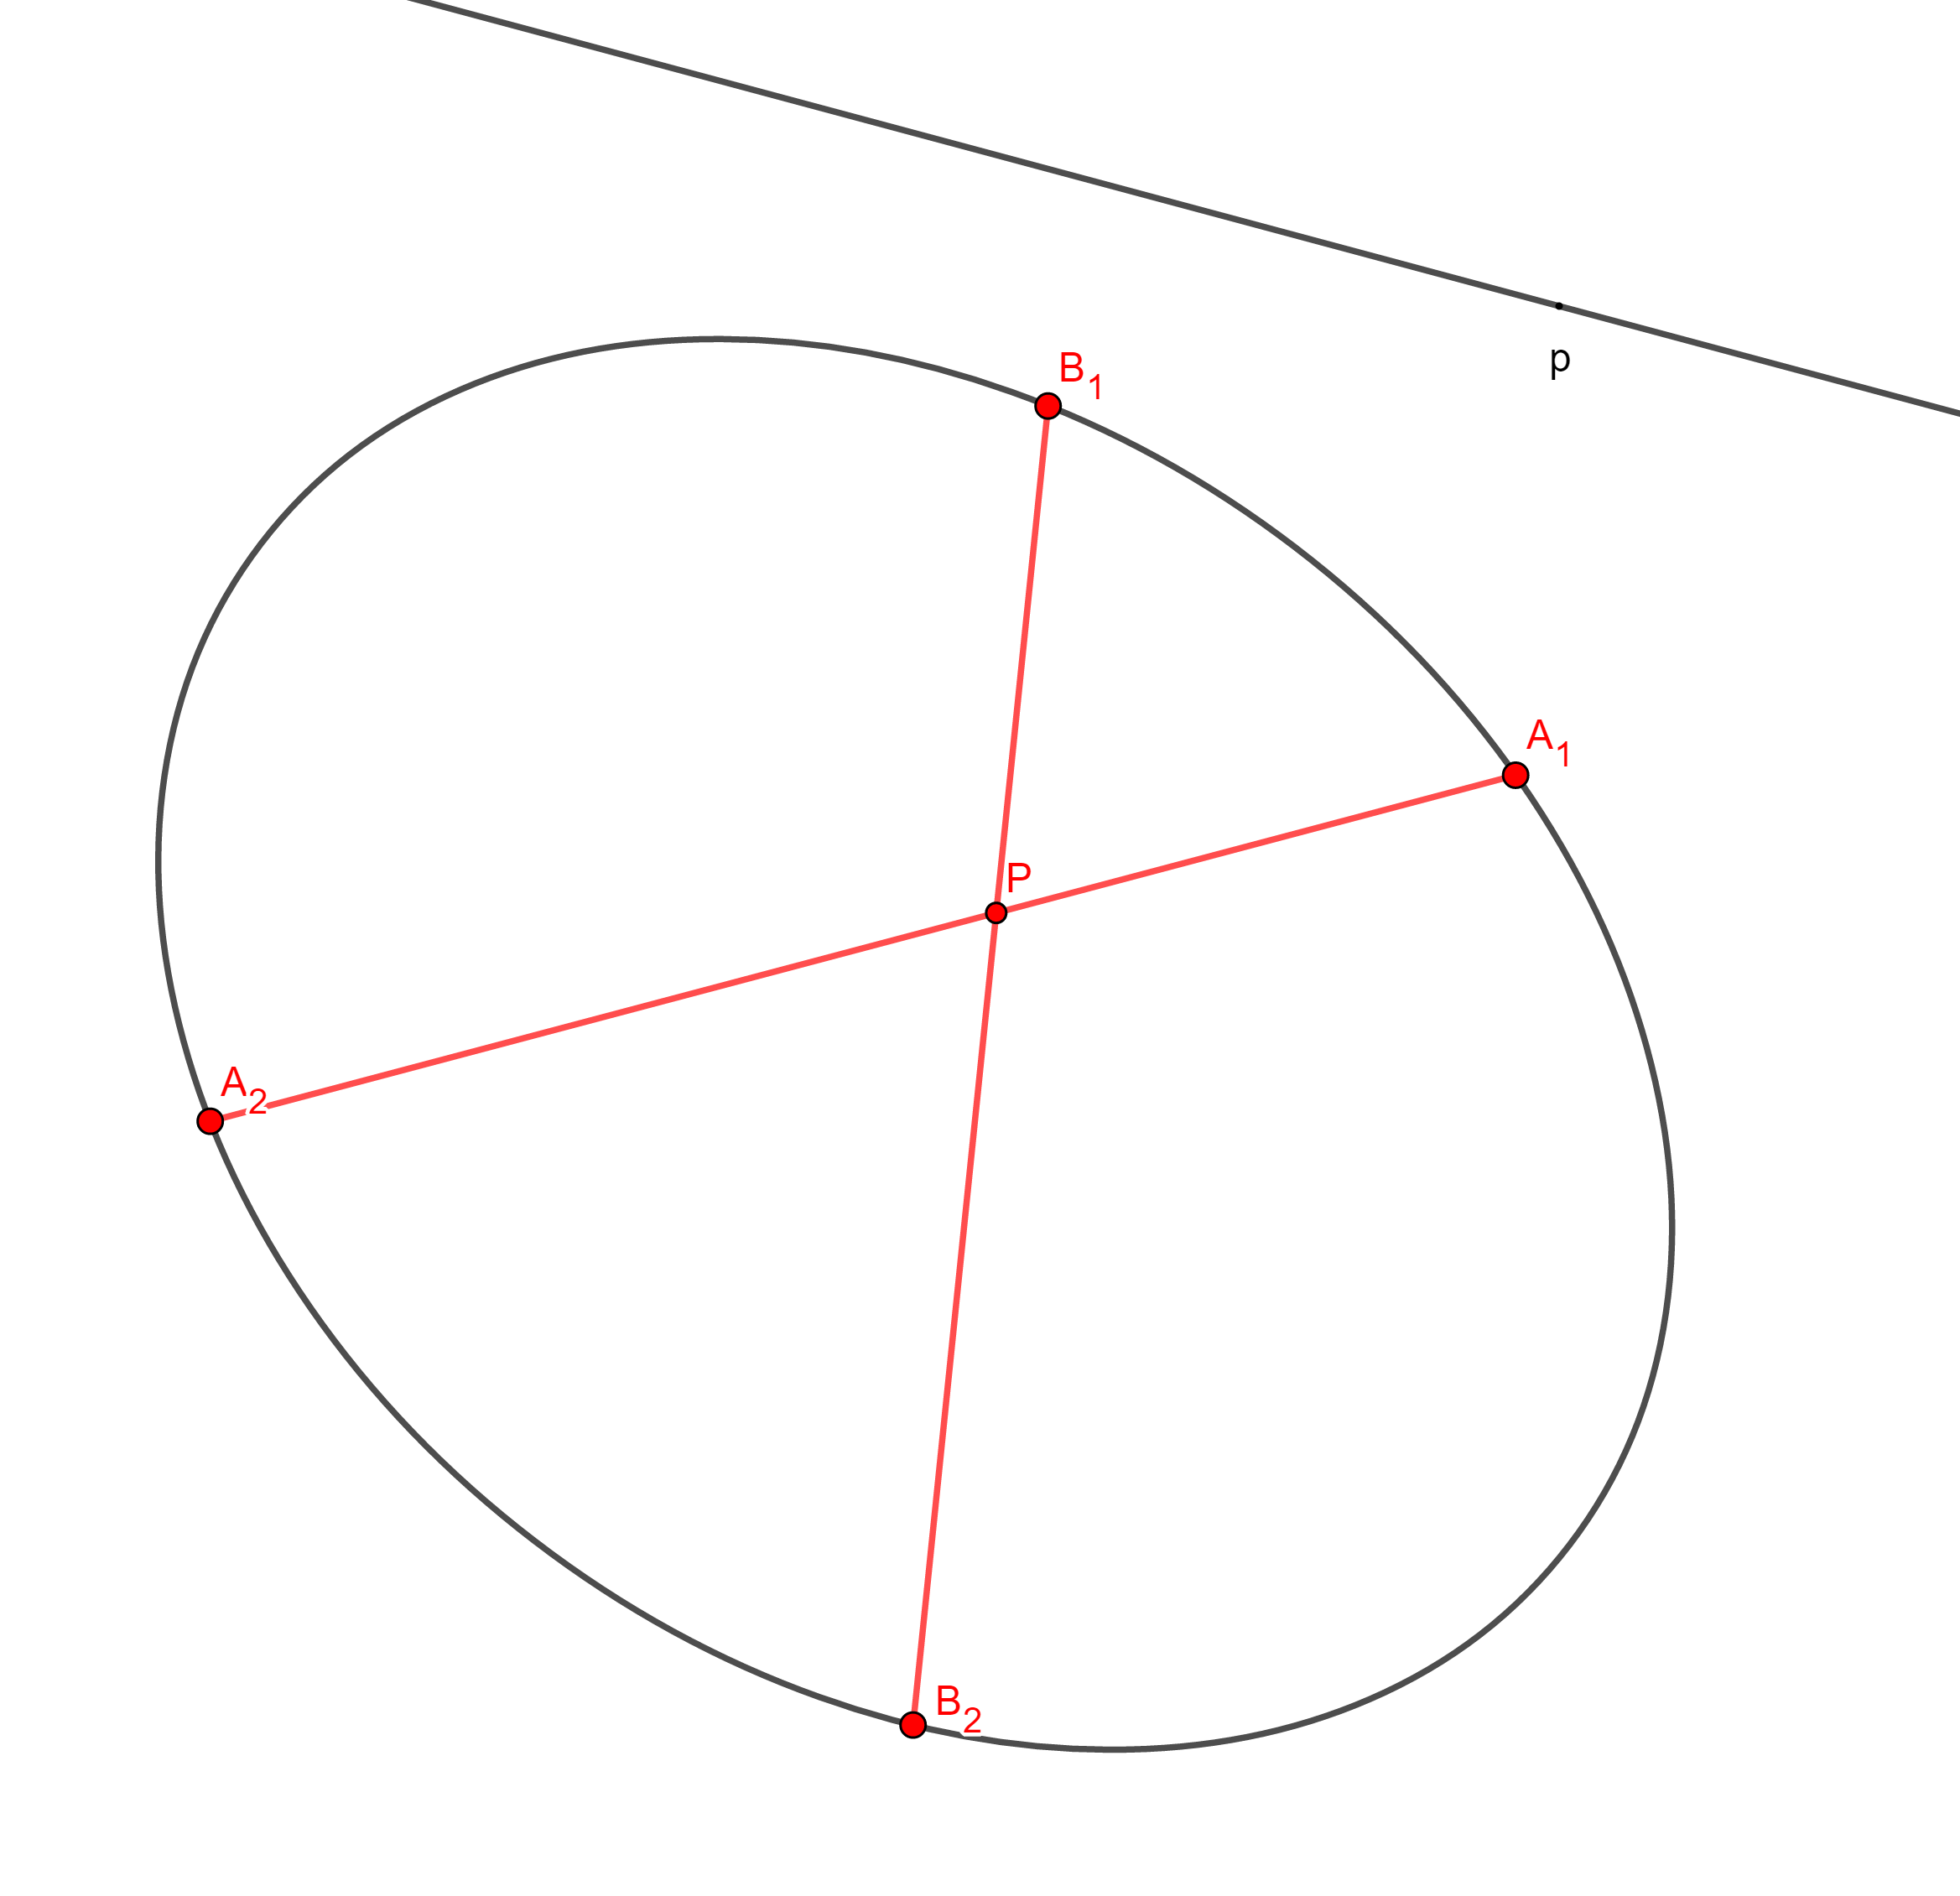
\includegraphics[width=0.8\linewidth]{pic13}}
			\end{minipage}
		\end{figure}
		
		
		\subsection*{3}
		\begin{figure}[h!]
			\center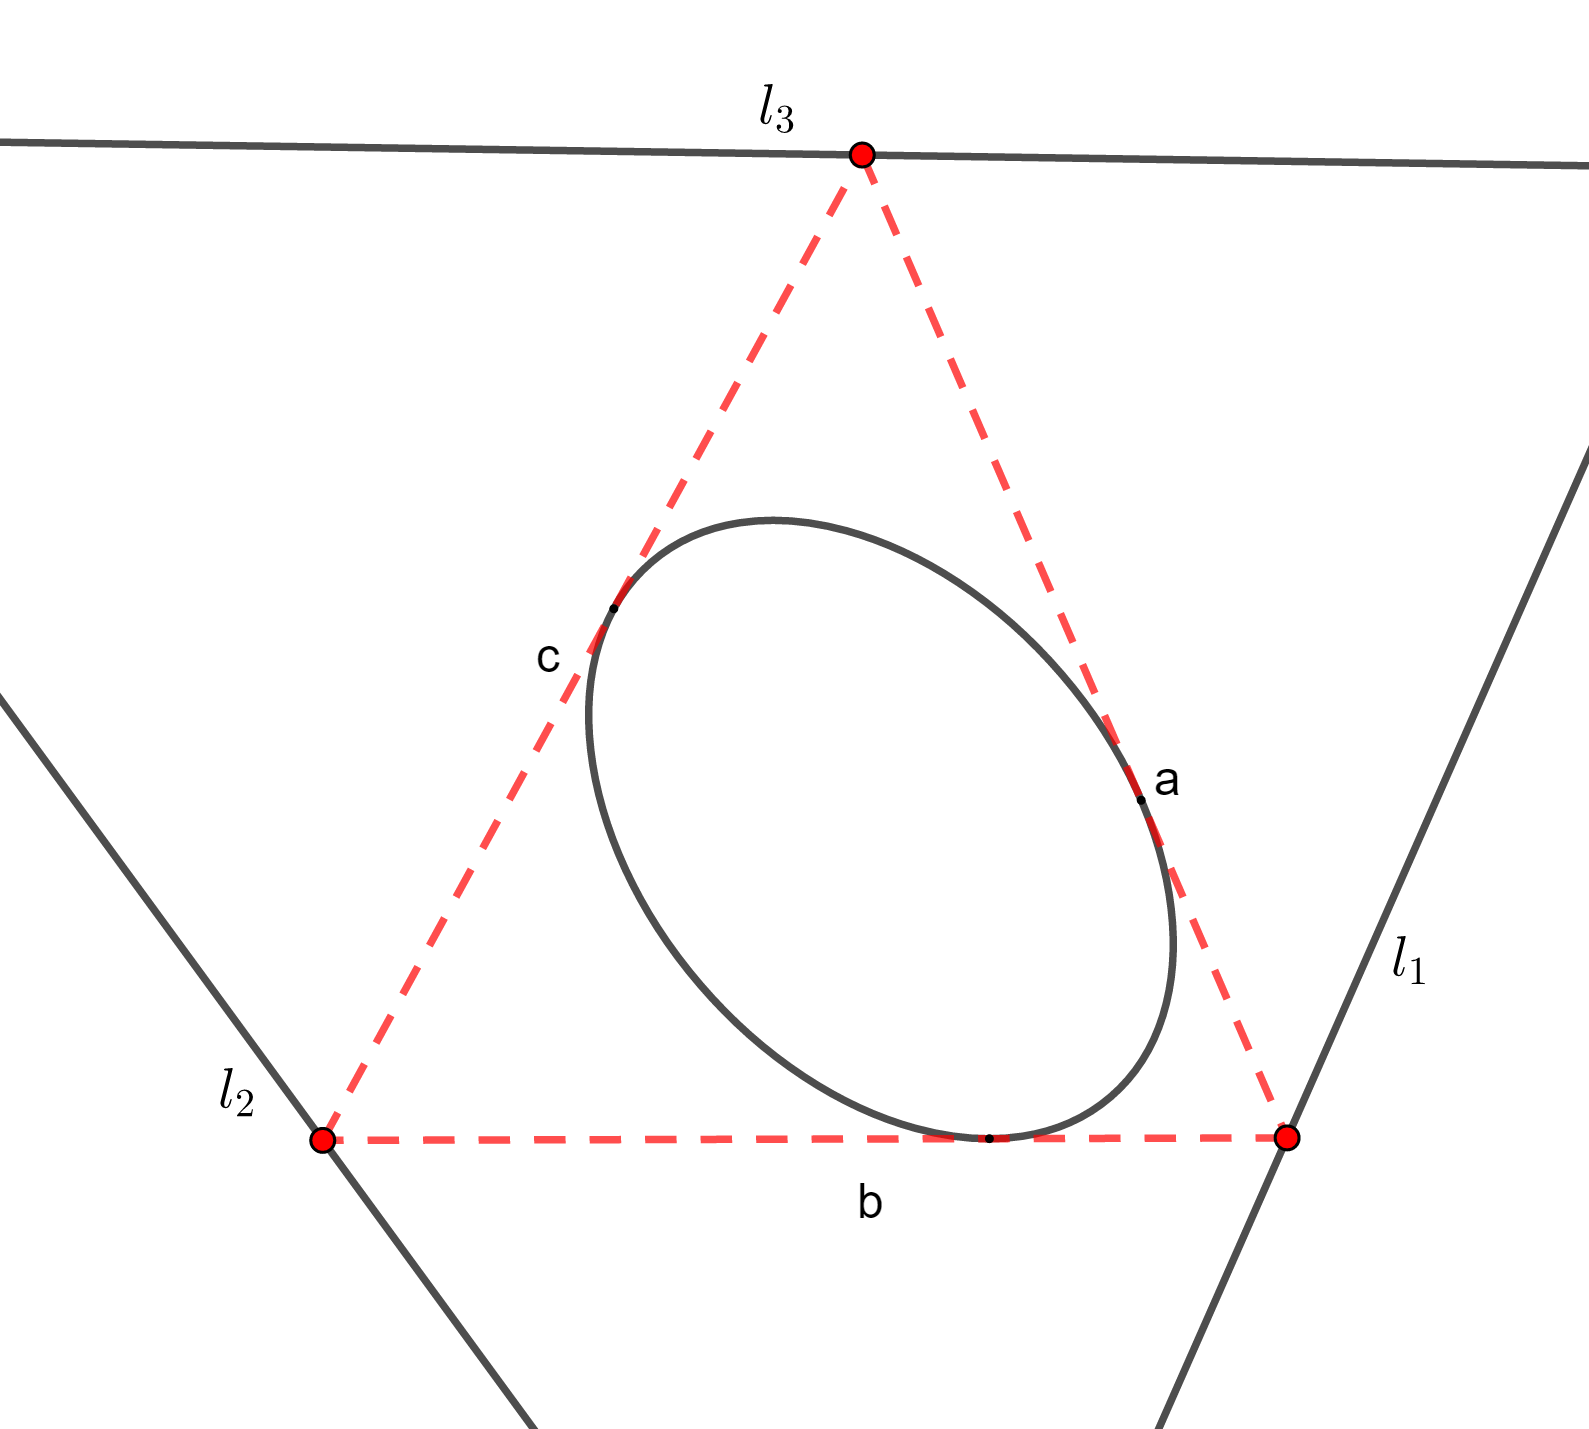
\includegraphics[width=0.4\linewidth]{pic14}
		\end{figure}
		
		\subsection*{4}